\documentclass[12pt, a4paper]{article}

% PACKAGES
\usepackage[margin=1in]{geometry} % Set page margins
\usepackage{amsmath}              % For advanced math environments
\usepackage{tikz}                 % For drawing diagrams
\usetikzlibrary{shapes.geometric} % For drawing stars and other shapes
\usepackage[colorlinks=true, urlcolor=blue, linkcolor=black]{hyperref} % For a clickable table of contents
\usepackage{graphicx}             % To scale tikz pictures if needed

% DOCUMENT INFORMATION
\title{\textbf{Problems on Projectile Motion on an Inclined Plane}}
\author{Generated by Gemini prompt by SiaLC}
\date{\today}

\begin{document}

\maketitle % Creates the title page

\newpage
\tableofcontents % Creates the table of contents

\newpage

% --------------------------------------------------------------------
% PROBLEM 1: RANGE ON AN INCLINED PLANE
% --------------------------------------------------------------------
\section{Range on an Inclined Plane}

\subsection{Question}
A projectile is fired from the base of an inclined plane of inclination $\beta = 30^{\circ}$. The initial velocity of the projectile is $v_0 = 100 \text{ m/s}$ at an angle $\alpha = 60^{\circ}$ with respect to the horizontal. Calculate the range of the projectile along the inclined plane. (Assume $g = 9.8 \text{ m/s}^2$).

\subsection{Explanation}
To solve this problem, we'll set up a coordinate system where the \textbf{x-axis is along the inclined plane} and the \textbf{y-axis is perpendicular to it}. The initial velocity $v_0$ and the acceleration due to gravity $g$ must be resolved into components along these new axes.
\begin{itemize}
    \item The angle of projection with respect to the inclined plane is $(\alpha - \beta)$.
    \item \textbf{Initial velocity components:}
        \begin{itemize}
            \item $v_{0x} = v_0 \cos(\alpha - \beta)$
            \item $v_{0y} = v_0 \sin(\alpha - \beta)$
        \end{itemize}
    \item \textbf{Acceleration components:}
        \begin{itemize}
            \item $a_x = -g \sin(\beta)$
            \item $a_y = -g \cos(\beta)$
        \end{itemize}
\end{itemize}
The \textbf{time of flight ($T$)} is the time taken for the projectile to return to the inclined plane, meaning its displacement in the y-direction is zero. The \textbf{range ($R$)} is the displacement in the x-direction during this time. The range can be calculated directly using the formula:
$$R = \frac{2v_0^2 \sin(\alpha - \beta) \cos(\alpha)}{g \cos^2(\beta)}$$

\subsection{Diagram}
\begin{center}
    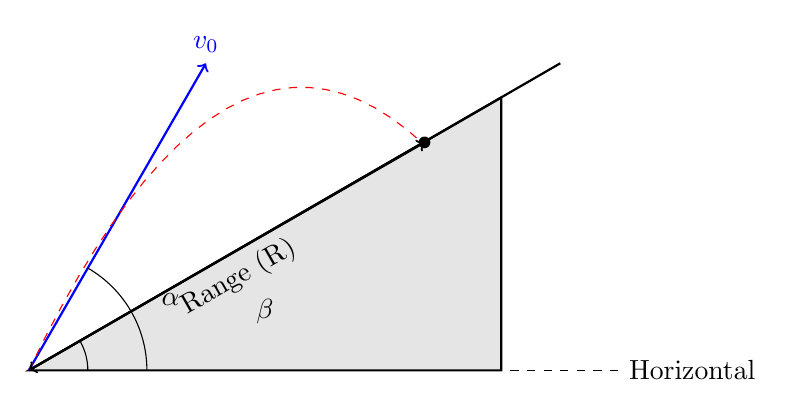
\begin{tikzpicture}[scale=1.5]
        % Draw the inclined plane
        \draw[thick, fill=gray!20] (0,0) -- (4,0) -- (4, 2.31) -- cycle;
        \draw[thick] (0,0) -- (4.5, 2.6);
        \node at (2, 0.5) {$\beta$};
        \draw (0.5,0) arc (0:30:0.5);

        % Draw the horizontal line
        \draw[dashed] (0,0) -- (5,0) node[right]{Horizontal};

        % Draw the projectile path
        \draw[blue, thick, ->] (0,0) -- (1.5, 2.6) node[above]{$v_0$};
        \draw[red, dashed, domain=0:3.35] plot (\x, {tan(30)*\x + 1.5*\x - 0.45*\x^2});

        % Mark the angle alpha
        \draw (1,0) arc (0:60:1);
        \node at (1.2, 0.6) {$\alpha$};
        
        % Mark the range R
        \coordinate (landing) at (3.35, 1.93); % Approx point on slope
        \draw[<->, thick] (0,0) -- (landing) node[midway, below, sloped]{Range (R)};
        \node at (landing) [circle, fill, inner sep=1.5pt]{};
    \end{tikzpicture}
\end{center}

\subsection{Solution}
Given values:
\begin{itemize}
    \item Initial velocity, $v_0 = 100 \text{ m/s}$
    \item Angle of projection with horizontal, $\alpha = 60^{\circ}$
    \item Angle of inclination of the plane, $\beta = 30^{\circ}$
    \item Acceleration due to gravity, $g = 9.8 \text{ m/s}^2$
\end{itemize}
We use the formula for the range on an inclined plane:
$$R = \frac{2v_0^2 \sin(\alpha - \beta) \cos(\alpha)}{g \cos^2(\beta)}$$
Substitute the values:
\begin{itemize}
    \item $\alpha - \beta = 60^{\circ} - 30^{\circ} = 30^{\circ}$
    \item $\cos(\alpha) = \cos(60^{\circ}) = 0.5$
    \item $\cos(\beta) = \cos(30^{\circ}) = \frac{\sqrt{3}}{2}$
\end{itemize}
$$R = \frac{2 \times (100)^2 \times \sin(30^{\circ}) \times \cos(60^{\circ})}{9.8 \times (\cos(30^{\circ}))^2}$$
$$R = \frac{2 \times 10000 \times 0.5 \times 0.5}{9.8 \times \left(\frac{\sqrt{3}}{2}\right)^2}$$
$$R = \frac{5000}{9.8 \times \frac{3}{4}} = \frac{5000}{7.35}$$
$$R \approx 680.27 \text{ meters}$$
The range of the projectile along the inclined plane is approximately \textbf{680.27 m}.

\newpage

% --------------------------------------------------------------------
% PROBLEM 2: ANGLE FOR MAXIMUM RANGE
% --------------------------------------------------------------------
\section{Angle for Maximum Range}

\subsection{Question}
A cannon is placed at the base of a hill with a slope of inclination $\beta = 15^{\circ}$. Determine the angle of projection $\alpha$ (with respect to the horizontal) that will result in the maximum possible range up the hill for a fixed initial velocity $v_0$.

\subsection{Explanation}
To find the angle that maximizes the range $R$, we need to find the maximum of the range formula with respect to the angle $\alpha$. The formula for range is:
$$R = \frac{2v_0^2 \sin(\alpha - \beta) \cos(\alpha)}{g \cos^2(\beta)}$$
Using the trigonometric identity $2 \sin(A)\cos(B) = \sin(A+B) + \sin(A-B)$, we can rewrite the numerator:
$$2 \sin(\alpha - \beta) \cos(\alpha) = \sin(\alpha - \beta + \alpha) + \sin(\alpha - \beta - \alpha) = \sin(2\alpha - \beta) - \sin(\beta)$$
So the range formula becomes:
$$R = \frac{v_0^2}{g \cos^2(\beta)} [\sin(2\alpha - \beta) - \sin(\beta)]$$
For a fixed $v_0$ and $\beta$, $R$ is maximum when $\sin(2\alpha - \beta)$ is maximum, which is 1.
$$\sin(2\alpha - \beta) = 1$$
$$2\alpha - \beta = \frac{\pi}{2} \quad (\text{or } 90^{\circ})$$
$$\alpha = \frac{\pi}{4} + \frac{\beta}{2}$$
This result shows that for maximum range, the angle of projection bisects the angle between the inclined plane and the vertical.

\subsection{Diagram}
\begin{center}
    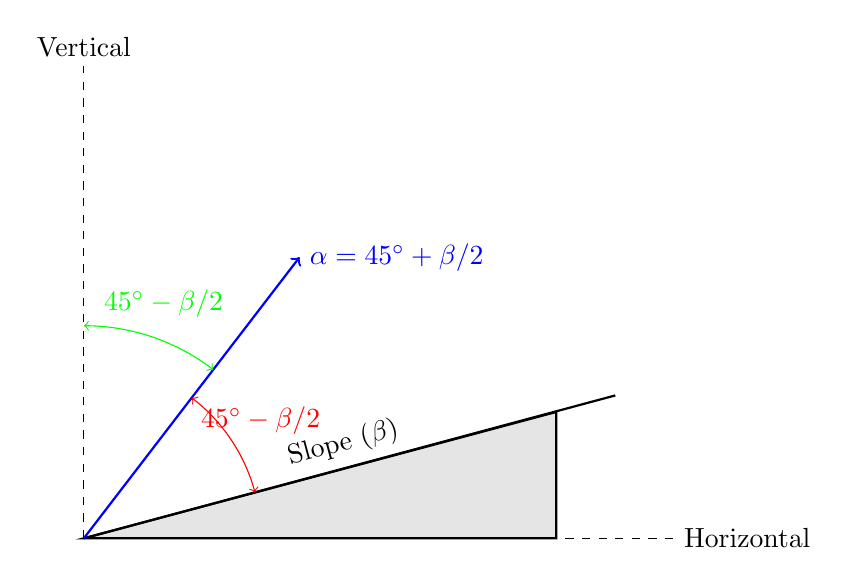
\begin{tikzpicture}[scale=1.5]
        % Draw the inclined plane
        \draw[thick, fill=gray!20] (0,0) -- (4,0) -- (4, 1.07) -- cycle;
        \draw[thick] (0,0) -- (4.5, 1.21) node[midway, above, sloped]{Slope ($\beta$)};
        
        % Draw the horizontal and vertical
        \draw[dashed] (0,0) -- (5,0) node[right]{Horizontal};
        \draw[dashed] (0,0) -- (0,4) node[above]{Vertical};
        
        % Angle of projection for max range
        \draw[blue, thick, ->, rotate=52.5] (0,0) -- (3,0) node[right]{$\alpha = 45^{\circ} + \beta/2$};
        
        % Show bisection
        % Angle between slope and bisector
        \draw[red, <->] (15:1.5) arc (15:52.5:1.5);
        \node[red] at (33.75:1.8) {$45^{\circ}-\beta/2$};
        
        % Angle between bisector and vertical
        \draw[green, <->] (52.5:1.8) arc (52.5:90:1.8);
        \node[green] at (71.25:2.1) {$45^{\circ}-\beta/2$};
    \end{tikzpicture}
\end{center}

\subsection{Solution}
Given the angle of inclination, $\beta = 15^{\circ}$. The condition for maximum range on an inclined plane is:
$$\alpha = \frac{90^{\circ}}{2} + \frac{\beta}{2}$$
$$\alpha = 45^{\circ} + \frac{15^{\circ}}{2}$$
$$\alpha = 45^{\circ} + 7.5^{\circ}$$
$$\alpha = 52.5^{\circ}$$
To achieve the maximum range up the hill, the cannon should be fired at an angle of \textbf{52.5°} to the horizontal.

\newpage

% --------------------------------------------------------------------
% PROBLEM 3: HITTING A MOVING TARGET
% --------------------------------------------------------------------
\section{Hitting a Moving Target on the Slope}

\subsection{Question}
A projectile is fired up an inclined plane of inclination $\beta = 30^{\circ}$ with an initial velocity $v_0 = 80 \text{ m/s}$ at an angle $\alpha = 60^{\circ}$ to the horizontal. Simultaneously, a target is released from rest from a point $L$ up the incline and begins to slide down with a constant acceleration of $a_T = 2.5 \text{ m/s}^2$. The projectile hits the target. Find the initial distance $L$. (Assume $g = 10 \text{ m/s}^2$).

\subsection{Explanation}
This problem requires us to find the point where the projectile and the target collide. The collision occurs if they are at the same place at the same time.
\begin{enumerate}
    \item \textbf{Calculate the Time of Flight (T):} First, we determine how long the projectile is in the air before it lands back on the slope. We use the motion perpendicular to the incline.
    $$y(t) = v_{0y}t + \frac{1}{2}a_y t^2$$
    The projectile lands when $y(T) = 0$.
    $$0 = (v_0 \sin(\alpha - \beta))T - \frac{1}{2}(g \cos(\beta))T^2$$
    Solving for $T \neq 0$:
    $$T = \frac{2 v_0 \sin(\alpha - \beta)}{g \cos(\beta)}$$
    \item \textbf{Calculate the Projectile's Range (R):} This is the distance the projectile travels along the incline during the time of flight $T$.
    $$R = v_{0x}T + \frac{1}{2}a_x T^2 = (v_0 \cos(\alpha - \beta))T - \frac{1}{2}(g \sin(\beta))T^2$$
    \item \textbf{Calculate Target's Distance ($S_T$):} This is the distance the target slides down the incline in the same time $T$. Since the target starts from rest ($u_T=0$):
    $$S_T = \frac{1}{2}a_T T^2$$
    \item \textbf{Find L:} The initial distance $L$ is the sum of the distance covered by the projectile up the slope and the distance covered by the target down the slope.
    $$L = R + S_T$$
\end{enumerate}

\subsection{Diagram}
\begin{center}
    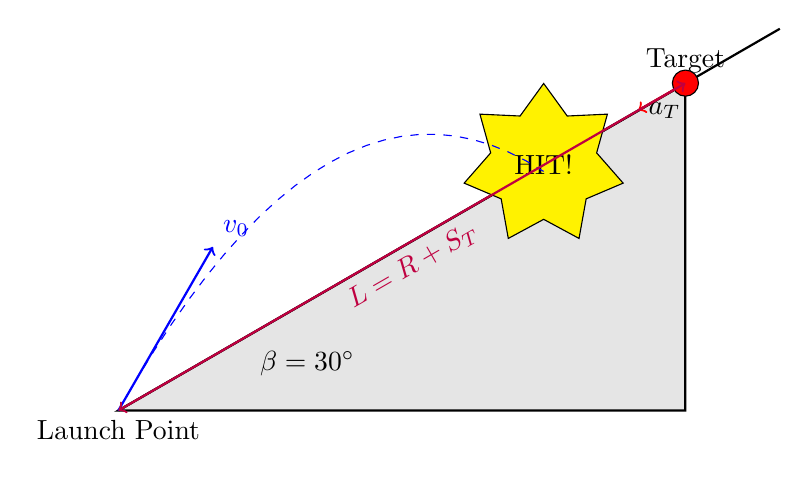
\begin{tikzpicture}[scale=1.2]
        % Draw the inclined plane
        \draw[thick, fill=gray!20] (0,0) -- (6,0) -- (6, 3.46) -- cycle;
        \draw[thick] (0,0) -- (7, 4.04);
        \node at (2, 0.5) {$\beta=30^{\circ}$};

        % Draw the horizontal line
        \draw[dashed] (0,0) -- (6,0);

        % Projectile
        \draw[blue, thick, ->] (0,0) -- (1, 1.732) node[above right]{$v_0$};
        \node[below] at (0,0) {Launch Point};
        
        % Target
        \coordinate (target_start) at (6, 3.464);
        \node[draw, circle, fill=red] at (target_start) {};
        \node[above] at (target_start) {Target};
        \draw[red, thick, ->] (target_start) --++ (-0.5, -0.288) node[right, black]{$a_T$};

        % Collision point
        \coordinate (collision) at (4.5, 2.598);
        \node[draw, star, star points=7, fill=yellow] at (collision) {HIT!};

        % Projectile path
        \draw[blue, dashed, domain=0:4.5] plot (\x, {tan(30)*\x + 1.2*\x - 0.27*\x^2});

        % Distance L
        \draw[<->, thick, purple] (0,0) -- (target_start) node[midway, below, sloped] {$L = R + S_T$};
    \end{tikzpicture}
\end{center}

\subsection{Solution}
Given values:
\begin{itemize}
    \item $v_0 = 80 \text{ m/s}$, $\alpha = 60^{\circ}$, $\beta = 30^{\circ}$
    \item $a_T = 2.5 \text{ m/s}^2$, $g = 10 \text{ m/s}^2$
\end{itemize}
\textbf{Step 1: Calculate the time of flight (T)}
$$T = \frac{2 v_0 \sin(\alpha - \beta)}{g \cos(\beta)} = \frac{2 \times 80 \times \sin(30^{\circ})}{10 \times \cos(30^{\circ})} = \frac{160 \times 0.5}{10 \times \frac{\sqrt{3}}{2}} = \frac{80}{5\sqrt{3}} = \frac{16}{\sqrt{3}} \text{ s}$$
\textbf{Step 2: Calculate the projectile's range (R)}
\begin{itemize}
    \item $v_{0x} = v_0 \cos(\alpha - \beta) = 80 \cos(30^{\circ}) = 40\sqrt{3} \text{ m/s}$
    \item $a_x = -g \sin(\beta) = -10 \sin(30^{\circ}) = -5 \text{ m/s}^2$
\end{itemize}
$$R = v_{0x}T + \frac{1}{2}a_x T^2 = (40\sqrt{3})\left(\frac{16}{\sqrt{3}}\right) + \frac{1}{2}(-5)\left(\frac{16}{\sqrt{3}}\right)^2$$
$$R = 640 - \frac{5}{2}\left(\frac{256}{3}\right) = 640 - \frac{640}{3} = \frac{1280}{3} \approx 426.67 \text{ m}$$
\textbf{Step 3: Calculate the distance the target travels ($S_T$)}
$$S_T = \frac{1}{2}a_T T^2 = \frac{1}{2}(2.5)\left(\frac{16}{\sqrt{3}}\right)^2 = 1.25 \times \frac{256}{3} = \frac{320}{3} \approx 106.67 \text{ m}$$
\textbf{Step 4: Find the initial distance L}
$$L = R + S_T = \frac{1280}{3} + \frac{320}{3} = \frac{1600}{3}$$
$$L \approx 533.33 \text{ m}$$
The initial distance between the launch point and the target was approximately \textbf{533.33 m}.

\newpage
% --------------------------------------------------------------------
% PROBLEM 4: COLLISION OF TWO PROJECTILES
% --------------------------------------------------------------------
\section{Collision of Two Projectiles on a Slope}

\subsection{Question}
Projectile A is fired from the base of an inclined plane of $\beta = 30^{\circ}$ with an initial velocity $v_A = 40 \text{ m/s}$ at an angle $\alpha = 60^{\circ}$ to the horizontal. Simultaneously, from a distance $L = 300 \text{ m}$ up the incline, Projectile B is fired horizontally with an initial velocity $v_B = 40 \text{ m/s}$ towards the base of the slope.

Show that the projectiles will collide and calculate the time and coordinates $(x, y)$ of the collision point relative to the base of the incline. (Assume $g = 10 \text{ m/s}^2$).

\subsection{Explanation}
This problem is best solved by analyzing the \textbf{relative motion} between the two projectiles. The key insight is that since both projectiles are subject to the same acceleration due to gravity ($\vec{g}$), their relative acceleration is zero.
$$\vec{a}_{rel} = \vec{a}_B - \vec{a}_A = (-g\hat{j}) - (-g\hat{j}) = \vec{0}$$
This means that the motion of one projectile as seen from the other is a straight line at a constant relative velocity.

A collision will occur if the initial relative velocity vector ($\vec{v}_{BA,0} = \vec{v}_{B,0} - \vec{v}_{A,0}$) is directed along the line connecting their initial positions (i.e., it is parallel to the initial relative position vector $\vec{r}_{BA,0} = \vec{r}_{B,0} - \vec{r}_{A,0}$).

The time of collision ($t_c$) can then be found using:
$$t_c = \frac{|\text{Initial Separation}|}{|\text{Relative Velocity}|} = \frac{|\vec{r}_{BA,0}|}{|\vec{v}_{BA,0}|}$$
Once the time is known, the collision coordinates can be found by plugging $t_c$ into the standard kinematic equations for either projectile. We will use a standard Cartesian coordinate system with the origin at the base of the slope.

\subsection{Diagram}
\begin{center}
    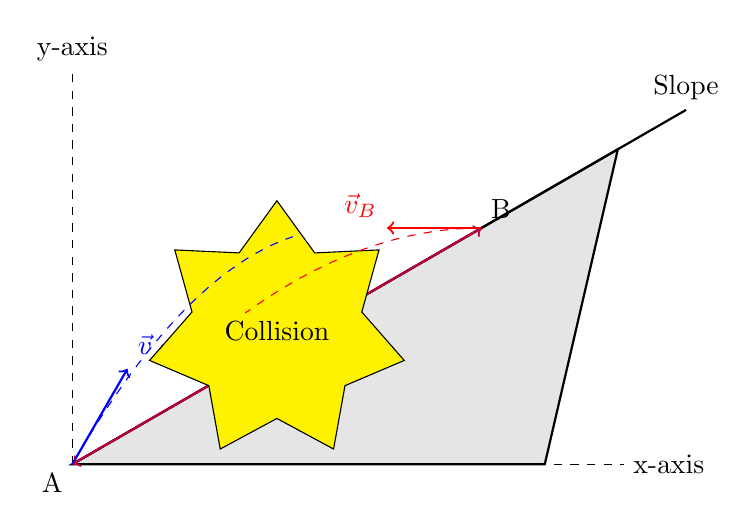
\begin{tikzpicture}[scale=1]
        % Draw the inclined plane and horizontal
        \draw[thick, fill=gray!20] (0,0) -- (6,0) -- (6.928, 4) -- cycle;
        \draw[thick] (0,0) -- (7.794, 4.5) node[above, sloped]{Slope};
        \draw[dashed] (0,0) -- (7,0) node[right]{x-axis};
        \draw[dashed] (0,0) -- (0,5) node[above]{y-axis};
        
        % Projectile A (from base)
        \node[below left] at (0,0) {A};
        \draw[blue, thick, ->] (0,0) -- (0.7, 1.212) node[above right]{$\vec{v}_A$};
        
        % Projectile B (from top)
        \coordinate (B_start) at (5.196, 3); % L=6m up the slope for diagram
        \node[above right] at (B_start) {B};
        \draw[red, thick, ->] (B_start) --++ (-1.2, 0) node[above left]{$\vec{v}_B$};
        
        % Draw initial separation vector L
        \draw[<->, thick, purple] (0,0) -- (B_start) node[midway, above, sloped] {$L$};

        % Collision point
        \coordinate (collision) at (2.598, 1.6875); % Scaled coordinates
        \node[draw, star, star points=7, fill=yellow] at (collision) {Collision};

        % Draw paths
        \draw[blue, dashed, domain=0:2.8] plot (\x, {1.732*\x - 0.25*\x^2});
        \draw[red, dashed, domain=0:3] plot ({5.196-\x}, {3 - 0.12*\x^2});
    \end{tikzpicture}
\end{center}

\subsection{Solution}
We set up a standard Cartesian coordinate system with the origin at the launch point of Projectile A.

\textbf{Step 1: Define Initial Position and Velocity Vectors}
\begin{itemize}
    \item \textbf{Projectile A:}
        \begin{itemize}
            \item $\vec{r}_{A,0} = 0\hat{i} + 0\hat{j}$
            \item $\vec{v}_{A,0} = (40 \cos 60^{\circ})\hat{i} + (40 \sin 60^{\circ})\hat{j} = 20\hat{i} + 20\sqrt{3}\hat{j} \text{ m/s}$
        \end{itemize}
    \item \textbf{Projectile B:}
        \begin{itemize}
            \item Position: $L=300$ m up a $30^{\circ}$ slope, so $x_{B,0} = 300 \cos 30^{\circ} = 150\sqrt{3}$ m and $y_{B,0} = 300 \sin 30^{\circ} = 150$ m.
            \item $\vec{r}_{B,0} = 150\sqrt{3}\hat{i} + 150\hat{j} \text{ m}$
            \item Velocity is horizontal towards the base: $\vec{v}_{B,0} = -40\hat{i} \text{ m/s}$
        \end{itemize}
\end{itemize}
\textbf{Step 2: Calculate Relative Vectors and Check for Collision}
\begin{itemize}
    \item Initial relative position: $\vec{r}_{BA,0} = \vec{r}_{B,0} - \vec{r}_{A,0} = 150\sqrt{3}\hat{i} + 150\hat{j}$
    \item Initial relative velocity: $\vec{v}_{BA,0} = \vec{v}_{B,0} - \vec{v}_{A,0} = (-40\hat{i}) - (20\hat{i} + 20\sqrt{3}\hat{j}) = -60\hat{i} - 20\sqrt{3}\hat{j}$
\end{itemize}
Check the ratio of components to see if the vectors are parallel:
\begin{itemize}
    \item Ratio for $\vec{r}_{BA,0}$: $\frac{y}{x} = \frac{150}{150\sqrt{3}} = \frac{1}{\sqrt{3}}$
    \item Ratio for $\vec{v}_{BA,0}$: $\frac{y}{x} = \frac{-20\sqrt{3}}{-60} = \frac{\sqrt{3}}{3} = \frac{1}{\sqrt{3}}$
\end{itemize}
The ratios are identical, so the vectors are parallel. \textbf{A collision will occur.}

\textbf{Step 3: Calculate the Time of Collision ($t_c$)}
$$t_c = \frac{|\vec{r}_{BA,0}|}{|\vec{v}_{BA,0}|}$$
\begin{itemize}
    \item $|\vec{r}_{BA,0}| = \sqrt{(150\sqrt{3})^2 + (150)^2} = 300 \text{ m}$ (This is $L$).
    \item $|\vec{v}_{BA,0}| = \sqrt{(-60)^2 + (-20\sqrt{3})^2} = \sqrt{3600 + 1200} = \sqrt{4800} = 40\sqrt{3} \text{ m/s}$.
\end{itemize}
$$t_c = \frac{300}{40\sqrt{3}} = \frac{15}{2\sqrt{3}} = \frac{5\sqrt{3}}{2} \text{ s} \approx 4.33 \text{ s}$$
\textbf{Step 4: Calculate the Collision Coordinates}
We use the equations of motion for Projectile A: $\vec{r}_A(t) = \vec{v}_{A,0}t + \frac{1}{2}\vec{g}t^2$.
\begin{itemize}
    \item $x_c(t) = (v_{A,0})_x t_c = 20 \times \left(\frac{5\sqrt{3}}{2}\right) = 50\sqrt{3} \text{ m}$
    \item $y_c(t) = (v_{A,0})_y t_c - \frac{1}{2}gt_c^2 = (20\sqrt{3})\left(\frac{5\sqrt{3}}{2}\right) - \frac{1}{2}(10)\left(\frac{5\sqrt{3}}{2}\right)^2$
    \item $y_c = 150 - 5\left(\frac{75}{4}\right) = 150 - \frac{375}{4} = \frac{225}{4} = 56.25 \text{ m}$
\end{itemize}
The collision occurs at time $\mathbf{t_c = \frac{5\sqrt{3}}{2}}$ s at coordinates $\mathbf{(50\sqrt{3} \text{ m}, 56.25 \text{ m})}$.

\end{document}